A evolu��o em n�mero de linhas de c�digos � mostrada na Figura~\ref{evolucao}. Parte dos dados dessa estat�stica para o simulador foi perdida por problemas no reposit�rio de arquivos. Apesar de n�o mostrar qu�o perto estamos do nosso objetivo, esse gr�fico ilustra as �pocas de maior atividade no projeto.

\begin{figure}[htbp]
\centering
\mbox{\subfigure[Linhas de c�digo do Simulador simulado]{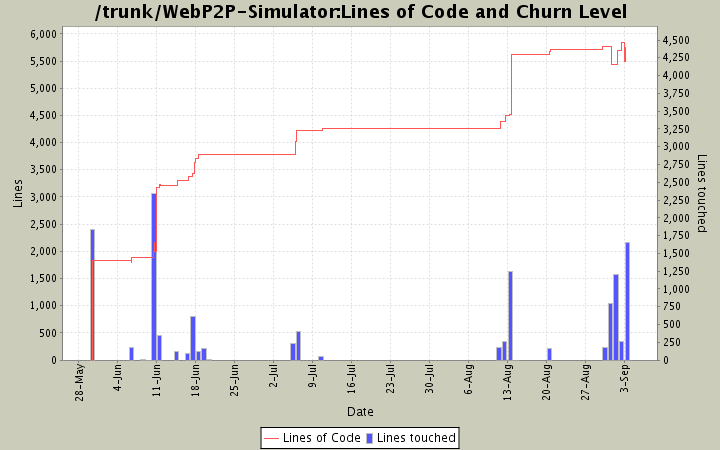
\includegraphics[width=7cm]{img/evolucaocodigosimulador.png}}

      \subfigure[N�mero de arquivos do Simulador]{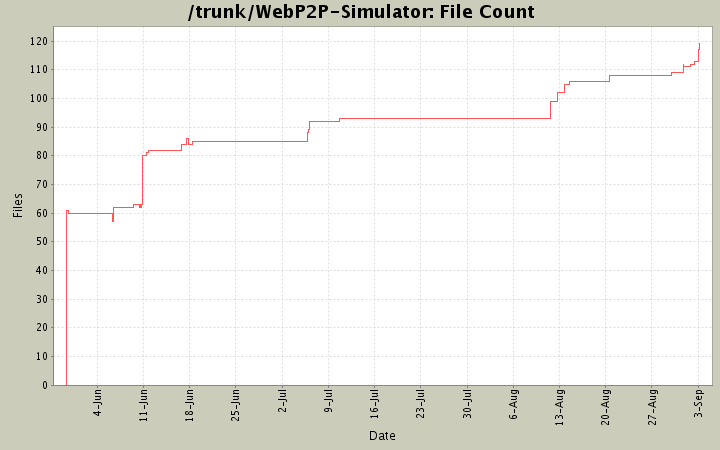
\includegraphics[width=7cm]{img/evolucaoarquivossimulador.png}}}

\mbox{\subfigure[Linhas de c�digo do Prot�tipo simulado]{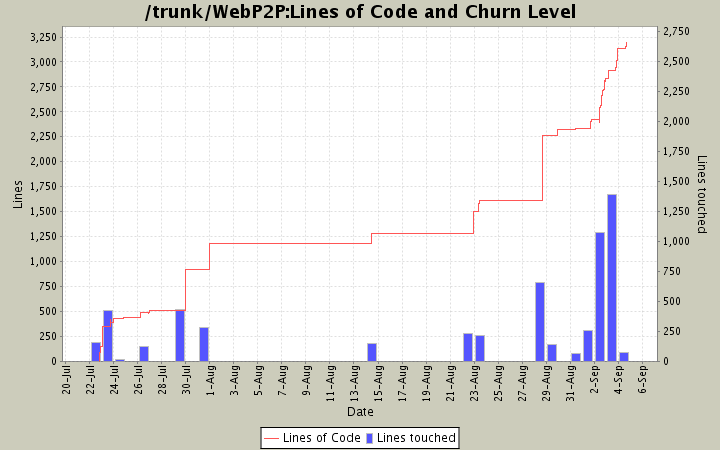
\includegraphics[width=7cm]{img/evolucaocodigo.png}}

      \subfigure[N�mero de arquivos do Prot�tipo]{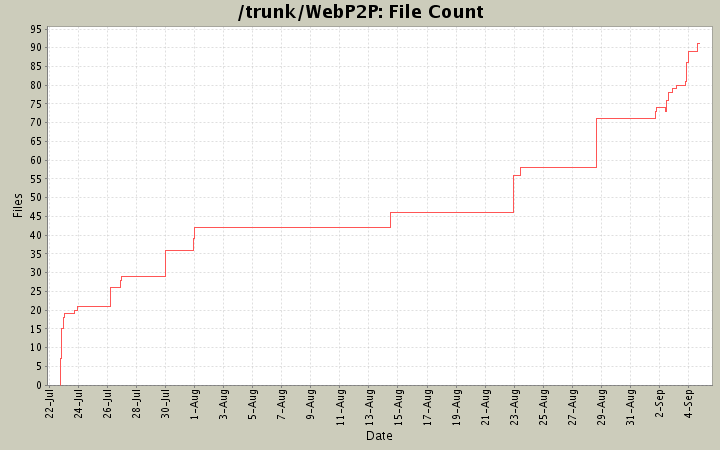
\includegraphics[width=7cm]{img/evolucaoarquivos.png}}}

\caption{Evolu��o do C�digo}
\label{evolucao}
\end{figure}

A m�trica ``linhas de c�digo'' n�o tem muita utilidade para o gerente do projeto, pois n�o o ajuda a prever e estimar prazos para cumprimento de tarefas. Foram criados Big Charts para ilustrar quando e quanto de cada atividade foi feita em uma determinada itera��o. A Figura~\ref{bigcharts} mostra esses gr�ficos tanto para a etapa de constru��o do simulador (Projeto 1) quanto para a de implementa��o do prot�tipo (Projeto 2).


\begin{figure}[htbp]
\centering
\mbox{\subfigure[Big Chart Projeto 1 simulado]{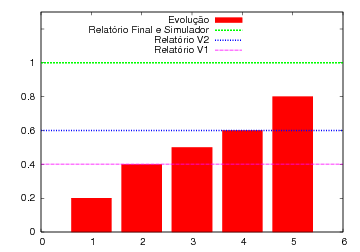
\includegraphics[width=7cm]{img/big_chart_projeto1.png}}

      \subfigure[Big Chart Projeto 2]{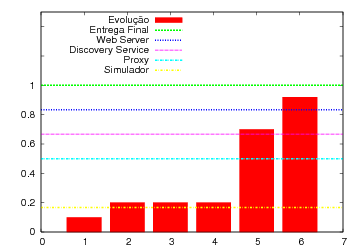
\includegraphics[width=7cm]{img/big_chart_projeto2.png}}}
\caption{Big Charts}
\label{bigcharts}
\end{figure}